% !TEX encoding = UTF-8
% !TEX TS-program = pdflatex
% !TEX root = ../tesi.tex

%**************************************************************
\chapter{Il contesto aziendale}
\label{cap:introduzione}
%**************************************************************

%\noindent Esempio di citazione in linea \\
%\cite{site:agile-manifesto}. \\

%**************************************************************
\section{Il profilo aziendale}

IT Euro Consulting \footcite{https://www.itecons.it} è un'azienda di medie dimensioni con sede legale a Padova, nata nel 2007 e facente parte del gruppo SCAI, presente su tutto il territorio italiano. 
Dalla sua nascita si è sempre occupata prevalentemente di consulenza, \textit{System Integration} ed \textit{Application Management}, in ambito ICT, operando in tutti i principali settori di mercato: bancario ed assicurativo, industria, pubblica amministrazione e servizi.
Nel corso degli anni l'azienda ha consolidato le proprie conoscenze, offrendo svariati servizi, soprattutto nei seguenti ambiti:
\begin{itemize}
	\item \textbf{Big Data}: supporto alle aziende nel loro processo di crescita e cambiamento, tramite moderne soluzioni di \textit{Business Intelligence} e la possibilità di prevedere scenari ed eventi futuri e prendere le più opportune decisioni operative o di business grazie all'analisi della gran mole di dati che ogni giorno vengono creati. Vengono quindi offerti servizi di \textit{big data engineer}, \textit{big data scientist}, \textit{big data architect} e \textit{big data administrator};
	\item \textbf{Internet of Things}: soluzioni \textit{end-to-end}, basate su tecnologie leader di mercato che consentono di indirizzare in modo efficace la realizzazione di sistemi IoT accelerando la realizzazione di componenti web e mobile per la raccolta, la visualizzazione e l’analisi dei dati;
	\item \textbf{Reference Architecture}: intesa come \textit{best practice} e struttura di base per un insieme di domini applicativi all’interno di un’organizzazione, la quale agevola il continuo allineamento dei processi e delle strategie con le giuste soluzioni tecnologiche. Vengono quindi offerti servizi di \textit{assessment}, design e consulenza;
	\item \textbf{DevOps}: automazione delle attività manuali nelle diverse fasi del \gls{SDLC}. Il modello DevOps non si concentra esclusivamente sull’ introduzione di nuovi tool, ma è inteso come una combinazione di cultura e processi unita agli strumenti di automazione. Vengono quindi offerti servizi di \textit{assessment} e consulenza; 
	\item \textbf{System Integration}: servizi di consulenza o interventi progettuali per aiutare le aziende a gestire al meglio le proprie strutture tecnologiche complesse e soluzioni applicative per semplificare la coesione fra i vari sottosistemi che compongono la struttura;
	\item \textbf{Application Management}: servizi di manutenzione correttiva, adattativa ed evolutiva di soluzioni applicative durante il loro intero ciclo di vita;
	\item \textbf{Customer Relationship Management}: con l'obiettivo di ottenere una visione completa per perseguire uno scenario di \gls{Single Customer View}, abilitante al dialogo \textit{one-to-one} tra l'organizzazione ed il proprio cliente indipendentemente dalle canalità attraverso le quali avviene l'interazione;
	\item \textbf{System \& Data Administration}: servizio consultivo svolto avvalendosi di un insieme di strategie, processi e regole che consentono di gestire i sistemi e trattare i dati fondamentali per lo sviluppo aziendale. Vengono quindi offerti servizi di \textit{database administration}, \textit{database security}, \textit{data governance}, \textit{data analysis} e \textit{scheduling management}.
\end{itemize}

I clienti principali di IT Euro Consulting sono aziende nazionali ed internazionali che lavorano nei seguenti settori:
\begin{itemize}
	\item \textit{\textbf{Banking}}
	\item \textit{\textbf{Insurance}}
	\item \textit{\textbf{Telecommunications}}
	\item \textit{\textbf{Media \& Technology}}
	\item \textit{\textbf{Public Administration}}
	\item \textit{\textbf{Utilities \& Energy}}
	\item \textit{\textbf{Manufacturing}}
\end{itemize}

%**************************************************************
\section{Tecnologie utilizzate}

Le tecnologie utilizzate dall'azienda per la realizzazione dei propri prodotti si possono raggruppare in due macro-sezioni, ovvero riguardanti lo sviluppo software e le attività inerenti ai \textit{big data}.
Per quanto concerne la prima, si può suddividere ulteriormente in due aree: \textit{back-end} e \textit{front-end}.

\subsection{Sviluppo software}
\textbf{Back-end}: buona parte del \textit{back-end} dei prodotti dell'azienda è scritta in linguaggio Java, in particolare utilizzando le specifiche fornite dalla versione \textit{Enterprise Edition}\footcite{https://www.oracle.com/technetwork/java/javaee}. Questa scelta è dovuta al grande supporto offerto da questo linguaggio in fatto di controllo degli accessi e sicurezza di applicativi delicati come quelli in ambito bancario e assicurativo;\\\\
\textbf{Front-end}: per quanto riguarda il \textit{front-end}, è utilizzato prevalentemente il \textit{framework} TypeScript Angular\footcite{https://angular.io/}, in quanto offre una grande elasticità d'impiego e buone prestazioni. \\

\subsection{Big Data}
\textbf{Hadoop}\footcite{https://hadoop.apache.org/}: \textit{framework} utilizzato per la gestione del \gls{cluster} e supporta applicazioni distribuite con elevato accesso ai dati, strutturati tramite il \textit{filesystem} chiamato HDFS. Permette alle applicazioni di lavorare con migliaia di nodi e petabyte di dati;\\
\textbf{Hive}\footcite{https://hive.apache.org/}: utilizzato per effettuare le \textit{query} e l'analisi preliminare dei dati in \textit{dataset} di grandi dimensioni;\\
\textbf{Impala}\footcite{https://impala.apache.org/}: simile ad Hive, ma fornisce prestazioni leggermente migliori a discapito di una minor affidabilità e peggior gestione degli errori; \\
\textbf{Spark}\footcite{https://spark.apache.org/}: \textit{framework} per il calcolo distribuito di dati strutturati in un \gls{cluster}. Supporta applicazioni scritte in molteplici linguaggi, quelli utilizzati in azienda sono principalmente Scala e Python;\\
\textbf{R}\footcite{https://www.r-project.org/}: linguaggio di programmazione e ambiente di sviluppo specifico per l'analisi statistica dei dati, utilizzato per la stima di modelli predittivi partendo dai dati ricavati utilizzando i precedenti strumenti;\\
\textbf{Python}\footcite{https://www.python.org/}: grazie alla sua elasticità ed ai suoi svariati utilizzi, Python è utilizzato anche per scopi analoghi al precedente strumento. Essendo la sintassi di questo linguaggio molto semplice, è ultimamente preferito a R.\\

%**************************************************************
\section{Processi aziendali}

L'azienda svolge il suo operato in base alla tipologia di lavoro da effettuare. Oltre ad eseguire progetti per un possibile cliente, sono attivi progetti per lo sviluppo di nuovo prodotto, dopo aver effettuato le ricerche di mercato d'interesse, da consegnare poi al reparto marketing per trovare compratori interessati; spesso, inoltre, vengono attivati dei progetti in seguito all'interesse relativo ad alcune gare d'appalto, principalmente per il settore privato ma in passato anche per quello pubblico.

\subsection{Metodologia di sviluppo}

\subsubsection{Sviluppo su commissione} \label{commissione}
Per quanto riguarda i progetti relativi allo sviluppo di un nuovo prodotto a seguito di una richiesta da parte del cliente, vengono eseguite le seguenti attività, supervisionate durante tutta la durata del progetto da un \textit{project manager} per coordinare i lavori ed interfacciarsi con il \textit{management} dell'azienda:
\begin{enumerate}
	\item \textbf{Analisi}: svolta in contemporanea dagli analisti e dal reparto marketing per il contatto con il cliente. Solitamente si cerca di partire da prodotti già sviluppati in azienda per poi personalizzarli in base alle richieste del cliente, così da poter offrire soluzioni già di base consolidate e testate in molteplici situazioni. Questo è preferibile soprattutto se le applicazioni sottostanti hanno bisogno di una maggior sicurezza, com'è il caso in ambito finanziario, anche per poter effettuare una manutenzione rapida in caso di malfunzionamenti.\\
	Il reparto marketing mantiene la maggior parte delle relazioni con il cliente finale all'inizio del rapporto, anche se un colloquio diretto di tecnici specializzati è ovviamente necessario dopo le prime interazioni per poter adottare soluzioni più specifiche e tecnicamente più complesse in base alle necessità del cliente;
	\item \textbf{Implementazione}: dopo aver identificato i requisiti assieme al cliente, il team incaricato si occupa dell'implementazione del prodotto concordato. Solitamente, per ogni progetto, sono assegnate un certo numero di persone e risorse per occuparsi del \textit{back-end} e del \textit{front-end} in base alla complessità ed alle tempistiche del progetto; in base alla tipologia ed alla necessità, questi saranno affiancati anche dal team che si occupa di \textit{big data} all'inizio dei lavori per le analisi sui dati necessari. Ogni team è supervisionato da un \textit{team leader} che mantiene il controllo sull'andamento dei lavori e le relazioni con gli altri team di sviluppo ed il \textit{project manager};
	\item \textbf{Rilascio}: dopo un'attenta attività di \textit{testing} interna all'azienda e di collaudo con il cliente, viene rilasciata una versione stabile del prodotto;
	\item \textbf{Manutenzione}: con il passare del tempo, il prodotto viene mantenuto e aggiornato secondo nuove specifiche del cliente o in seguito a problemi riscontrati, sia sul singolo prodotto sia in caso di problemi in prodotti che condividono la stessa base di partenza e quindi passibili degli stessi errori che potrebbero compromettere la stabilità e la sicurezza.
\end{enumerate}

\subsubsection{Sviluppo nuovo prodotto}
Nel caso il prodotto non sia precedentemente commissionato da un cliente, le attività che vengono seguite sono leggermente differenti. Il reparto di ricerca e sviluppo, il team \textit{big data} ed il reparto marketing collaborano alla ricerca di un prodotto appetibile per un eventuale cliente a cui verrà in genere presentato solamente un \textit{\gls{MVP}}: in questo modo è possibile presentare all'interessato un prototipo del prodotto con alcune funzionalità essenziali e significative, senza perdite inutili di tempo e risorse per l'azienda. Le attività di implementazione, rilascio e manutenzione che sono eseguite in seguito all'ottenimento di un cliente interessato sono invece pari a quelle dello \hyperref[commissione]{sviluppo su commissione}.
\begin{figure}[!h] 
	\centering 
	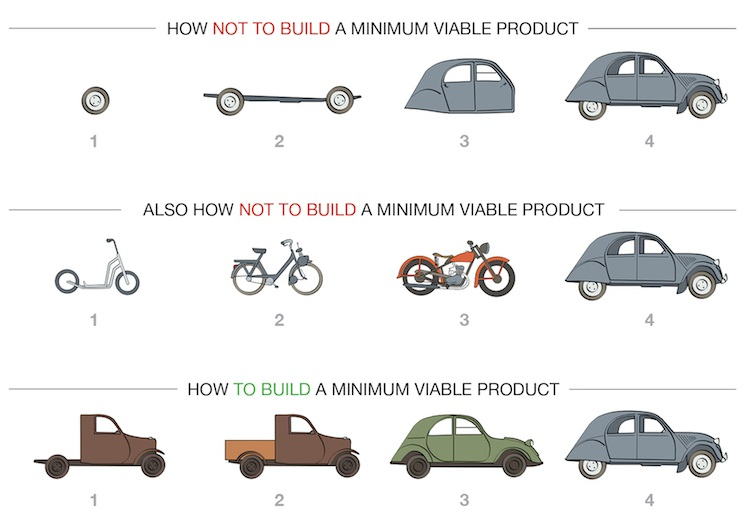
\includegraphics[width=0.9\columnwidth]{MVP} 
	\caption{Framework to build an MVP: Minimum Viable Product (goo.gl/s8LmEH)}
	
	
	
\end{figure}

\subsection{Controllo di versione}
Come strumento di versionamento del codice, l’azienda utilizza \gls{Git}\footcite{https://git-scm.com/} ed in particolare, per poter gestire tutto il codice derivante dai vari progetti, viene utilizzata la versione \textit{enterprise} di \gls{GitLab}\footcite{https://about.gitlab.com/}, disponibile gratuitamente sotto licenza \textit{open source}.\\
Alcuni dei vantaggi che ha spinto l’azienda ad utilizzare Git sono:
\begin{itemize}
	\item \textbf{Ridondanza}: ogni sviluppatore possiede una copia dell’intera \textit{repository}. Il rischio di perdita dei sorgenti del progetto è quindi inversamente proporzionale al numero di sviluppatori che ne possiedono in locale l’ultima versione; in caso di perdita del progetto di uno sviluppatore quindi si andrà incontro solamente alla perdita delle ultime modifiche personali fatte;
	\item \textbf{Disponibilità}: anche in assenza di connessione alla \textit{repository} principale, è possibile continuare ad effettuare \textit{commit} ed a salvare le modifiche fatte nel tempo. Una volta ripristinata la connessione, la \textit{repository} locale può essere sincronizzata con quella remota rendendo le modifiche disponibili a tutti;
	\item \textit{\textbf{Branch e Merge}}: permette con molta facilità la creazione di \textit{branch}, consentendo di creare quindi delle ramificazioni in cui sviluppare funzionalità non stabili, evitando di intaccare il ramo principale dove di norma risiede una versione stabile e testata del prodotto. Nel momento in cui si vogliono salvare le modifiche anche nel ramo principale, \gls{Git} permette di effettuare l’operazione di \textit{merge} del nuovo ramo testato con il ramo principale e considerare quindi le ultime modifiche come stabili;
	\item \textit{\textbf{Fork e Pull request}}: queste due operazioni permettono di clonare una \textit{repository} (tramite \textit{fork}) e, successivamente, proporre l’inclusione delle modifiche apportate all’interno del clone nella \textit{repository} originale.
\end{itemize}

\subsection{Ambiente di sviluppo}
Gli strumenti utilizzati per lo sviluppo, divisi in categorie, sono i seguenti:
\begin{itemize}
	\item \textbf{IntelliJ IDEA}\footcite{https://www.jetbrains.com/idea/}: è l'\gls{IDE} utilizzato in prevalenza dagli sviluppatori in quanto supporta vari linguaggi di programmazione e vari tool utili;
	\item \textbf{Visual Studio Code}\footcite{https://code.visualstudio.com/}: come il precedente, supporta vari linguaggi di programmazione e molteplici estensioni volte a migliorare lo sviluppo. A differenza del precedente, però, non supporta nativamente Java ed è quindi meno utilizzato;
	\item \textbf{\gls{Bash}}: per effettuare l'analisi dei dati preliminari da parte del team \textit{big data} viene utilizzata la \textit{shell} di Linux per eseguire i tool interessati (ad esempio Hive, Impala, Spark o per visualizzare il \textit{filesystem} HDFS).
\end{itemize}

%**************************************************************
\section{Propensione dell'azienda per l'innovazione}
L’azienda è alla continua ricerca di nuove tecnologie e prodotti innovativi che possano soddisfare sempre più le esigenze del cliente. Nel primo caso l’azienda cerca di cogliere il meglio delle nuove tecnologie per poterne trarre il maggior beneficio possibile attraverso progetti sperimentali e, per la prima volta quest’anno, stage universitari. Essendo l’innovazione un importante fattore di crescita, IT Euro Consulting coltiva questo aspetto cercando personale che abbia attitudine al cambiamento e contemporaneamente esprima le proprie soluzioni ai problemi incontrati dando libero sfogo alla propria creatività. Nel secondo caso, invece, l’azienda si prefigge l’obiettivo di creare nuovi prodotti al passo con le esigenze di potenziali clienti, utilizzando le ultime tecnologie disponibili.\\
Un'ulteriore prova della propensione all'innovazione dell'azienda è la presenza di un team specifico ed in continua espansione per il segmento \textit{big data}, cosa usuale all'estero ma ben più rara in Italia in aziende di medie dimensioni, nelle quali l'importanza dei dati e della potenzialità che essi possiedono non è ancora entrata pienamente nell'ideale di business delle aziende.

%**************************************************************